\documentclass[Thesis.tex]{subfiles}
\begin{document}

\chapter{{\sc VaryLab} - Discrete surface optimization}
\label{chp:varylab}

\section{Introduction}

\begin{figure}
\begin{center}
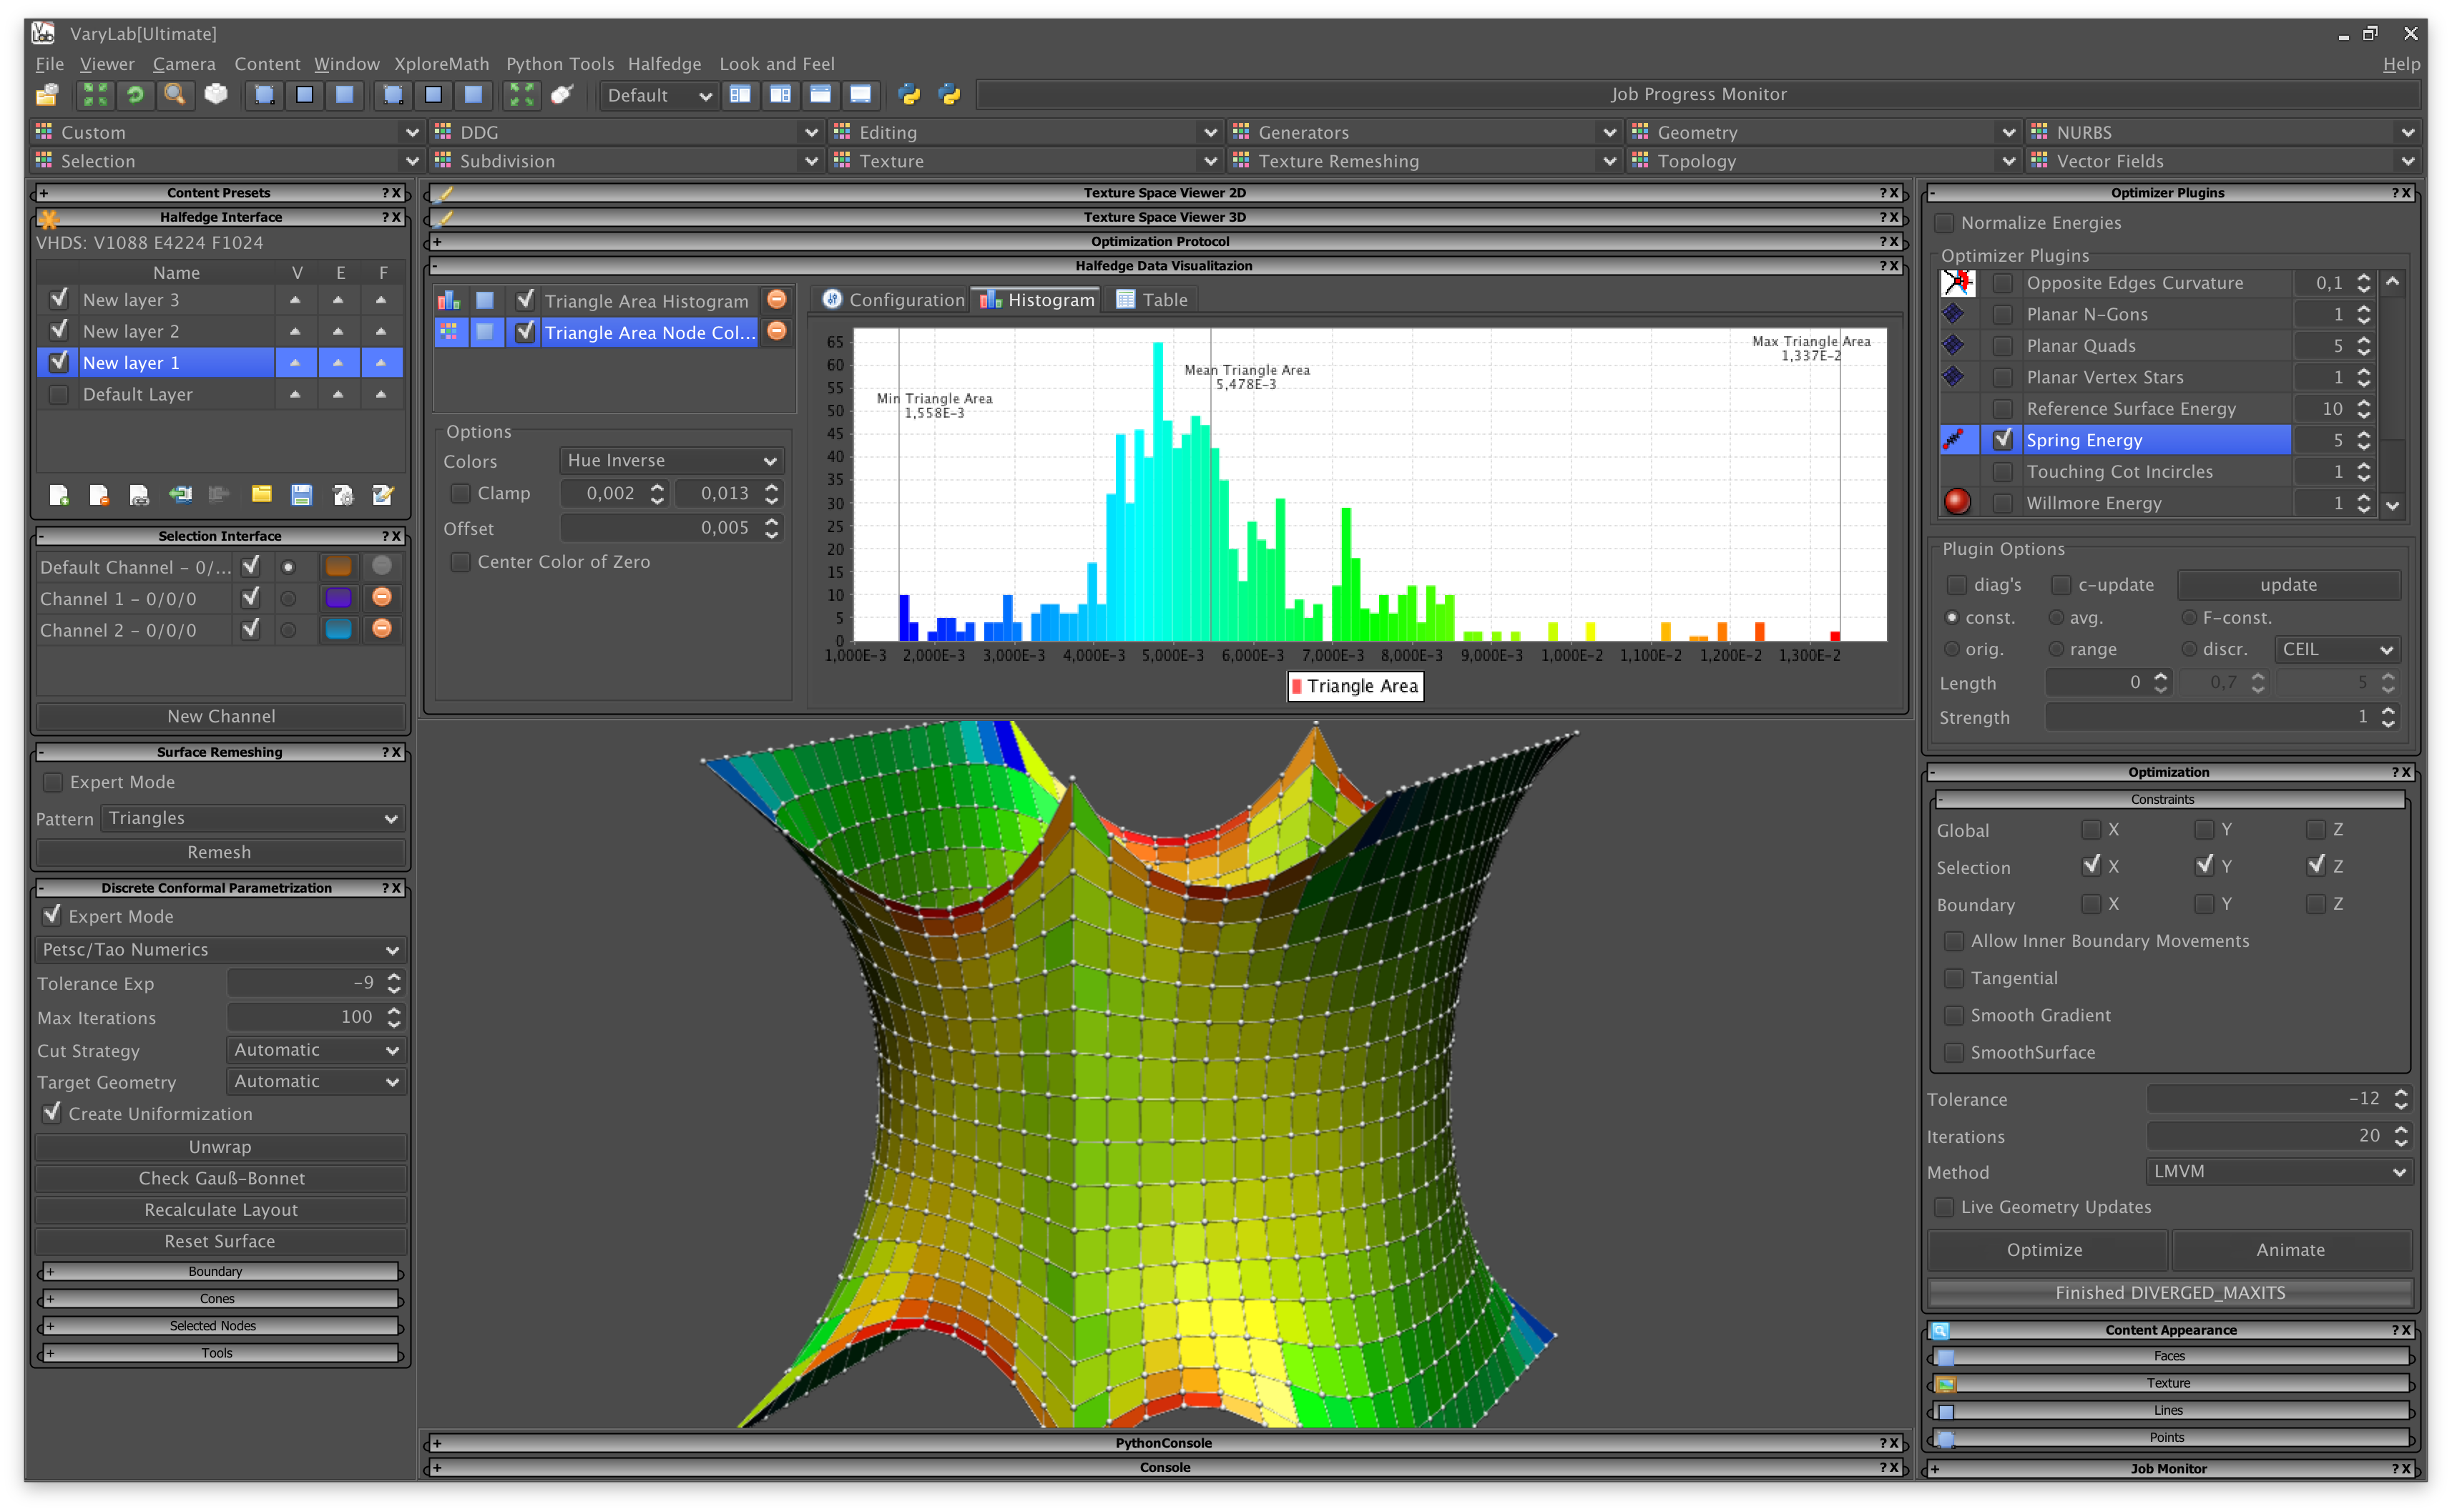
\includegraphics[width=\textwidth]{varylab/varylab_main.png}
\caption{{\sc VaryLab} user interface.}
\label{fig:varylab_main_ui}
\end{center}
\end{figure}

\section{User interface}

The user interface of {\sc VaryLab} is decided into 

\begin{figure}
\begin{center}
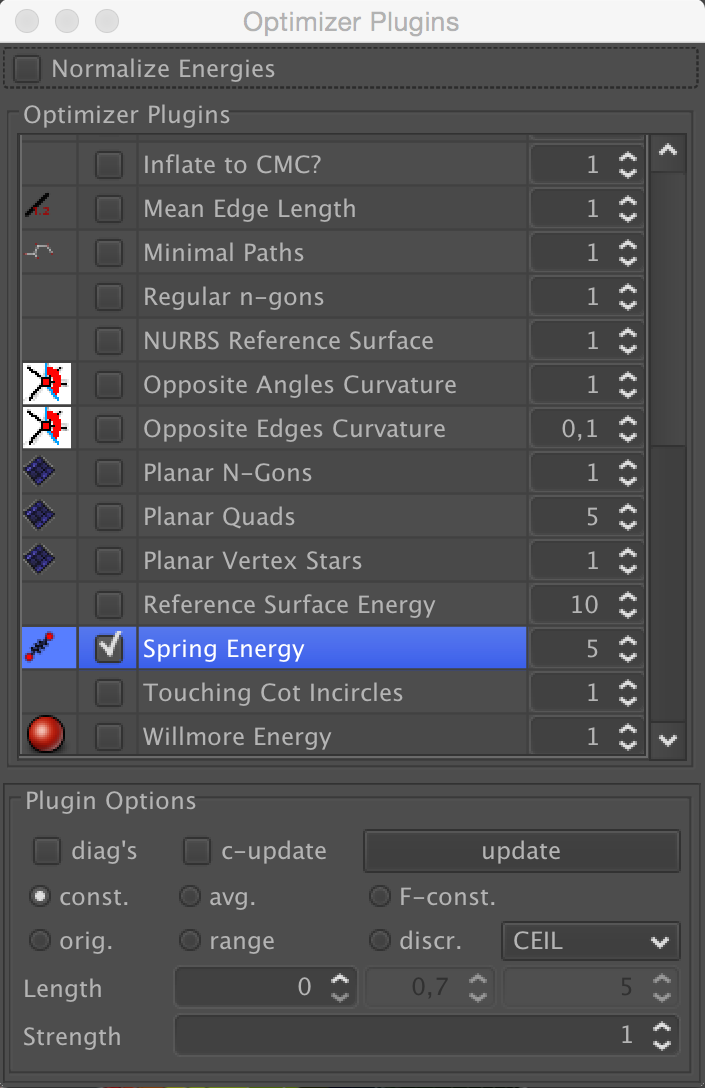
\includegraphics[width=0.5\textwidth]{varylab/optimization_plugins.png}\hfill
\begin{minipage}[b]{0.47\linewidth}
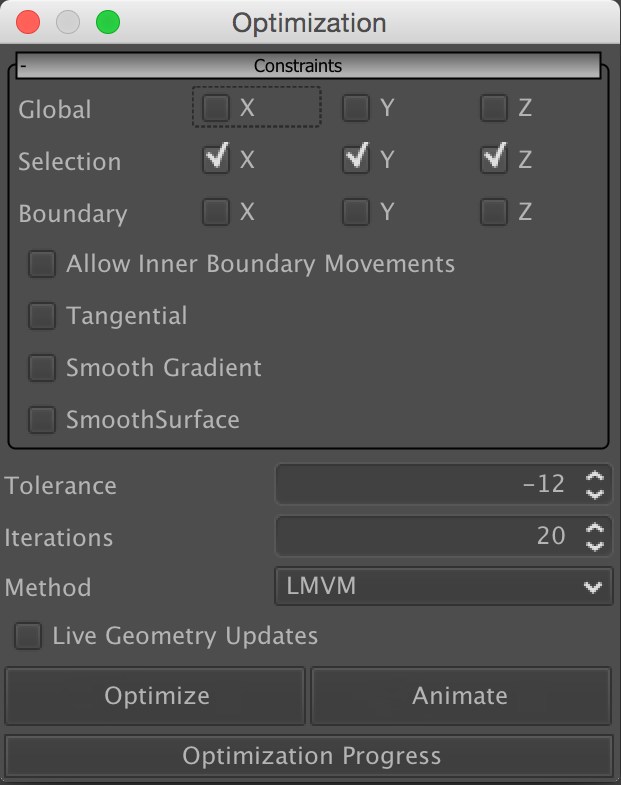
\includegraphics[width=\linewidth]{varylab/optimization.png}\\
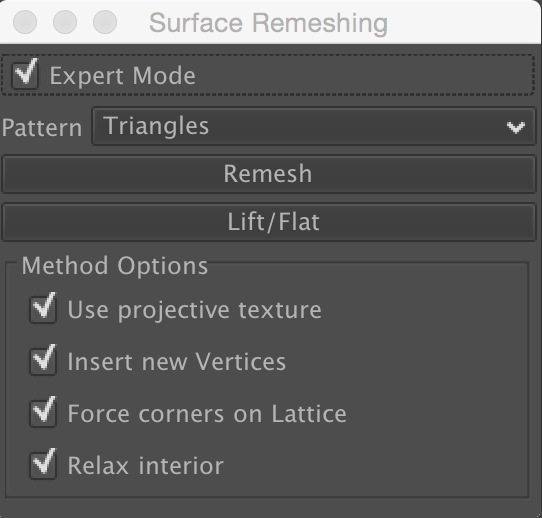
\includegraphics[width=\linewidth]{varylab/remeshing.png}
\end{minipage}\\
\vskip 0.05cm
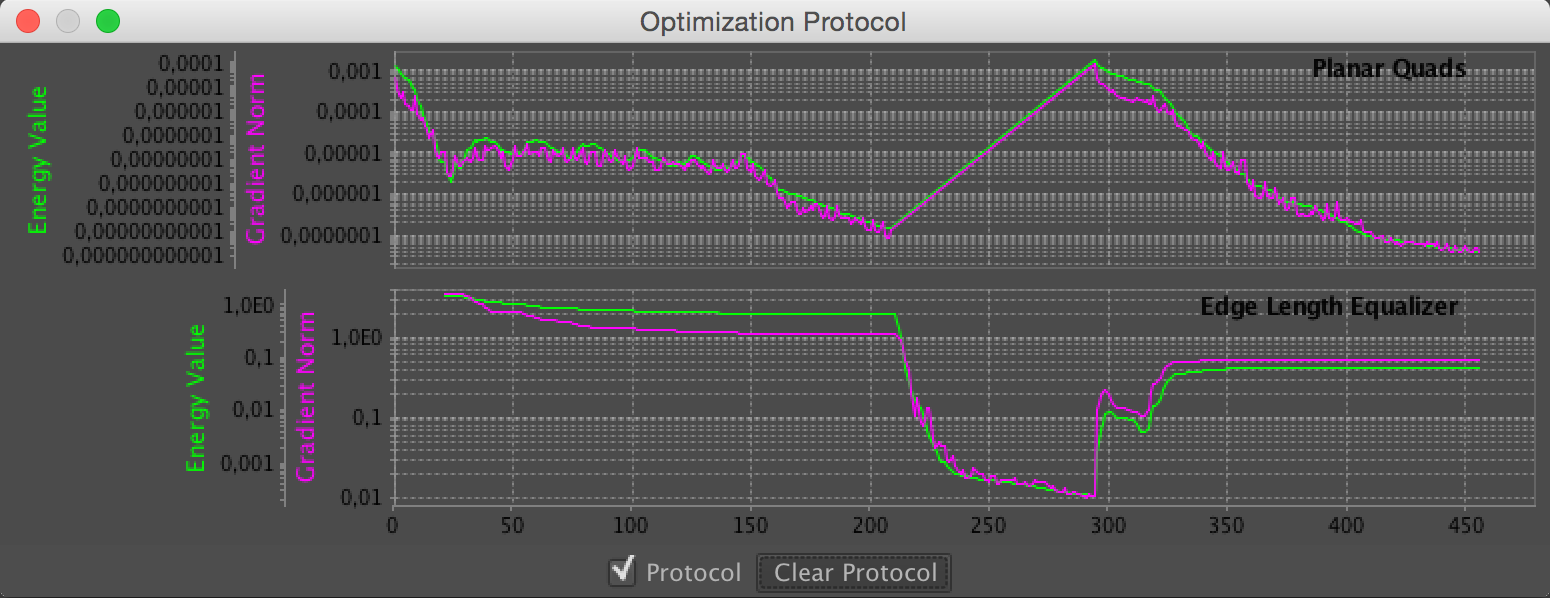
\includegraphics[width=\textwidth]{varylab/protocol.png}
\caption{The main user interface panels of {\sc VaryLab}. List of optimization functional plug-ins and their options (left). Main optimization controls with global constraints and minimizer settings (top right). Remeshing ui for different patterns (right middle). Optimization protocol panel (bottom) shows the progress of the optimization for each activated energy.}
\label{default}
\end{center}
\end{figure}



\section{{\sc VaryLab[Service]}}

\section{{\sc U3D} - 3D content in presentations and online publications}
\label{sec:u3d}

\subfilebibliography
\end{document}

%%% Local Variables:
%%% TeX-master: "Thesis.tex"
%%% End: